% mnras_template.tex
%
% LaTeX template for creating an MNRAS paper
%
% v3.0 released 14 May 2015
% (version numbers match those of mnras.cls)
%
% Copyright (C) Royal Astronomical Society 2015
% Authors:
% Keith T. Smith (Royal Astronomical Society)

% Change log
%
% v3.0 May 2015
%    Renamed to match the new package name
%    Version number matches mnras.cls
%    A few minor tweaks to wording
% v1.0 September 2013
%    Beta testing only - never publicly released
%    First version: a simple (ish) template for creating an MNRAS paper

%%%%%%%%%%%%%%%%%%%%%%%%%%%%%%%%%%%%%%%%%%%%%%%%%%
% Basic setup. Most papers should leave these options alone.
\documentclass[a4paper,fleqn,usenatbib]{mnras}

% MNRAS is set in Times font. If you don't have this installed (most LaTeX
% installations will be fine) or prefer the old Computer Modern fonts, comment
% out the following line
\usepackage{newtxtext,newtxmath}
% Depending on your LaTeX fonts installation, you might get better results with one of these:
%\usepackage{mathptmx}
%\usepackage{txfonts}

% Use vector fonts, so it zooms properly in on-screen viewing software
% Don't change these lines unless you know what you are doing
\usepackage[T1]{fontenc}
\usepackage{ae,aecompl}

%%%%% AUTHORS - PLACE YOUR OWN PACKAGES HERE %%%%%

% Only include extra packages if you really need them. Common packages are:
\usepackage{graphicx}	% Including figure files
\usepackage{amsmath}	% Advanced maths commands
\usepackage{amssymb}	% Extra maths symbols
\usepackage[xindy]{glossaries}
\glsdisablehyper
\usepackage{subcaption}
\usepackage{tabularx}
\captionsetup{compatibility=false}
\usepackage[normalem]{ulem}

%%%%%%%%%%%%%%%%%%%%%%%%%%%%%%%%%%%%%%%%%%%%%%%%%%

%%%%% AUTHORS - PLACE YOUR OWN COMMANDS HERE %%%%%

% Please keep new commands to a minimum, and use \newcommand not \def to avoid
% overwriting existing commands. Example:
%\newcommand{\pcm}{\,cm$^{-2}$}	% per cm-squared

\newcommand{\GSF}[1]{\noindent\textcolor{blue}{GSF:#1}}
%comments by Marisa
\newcommand{\cM}[1]{\textcolor{magenta}{ #1 --M}}

%glossary
\newacronym{alfa}{ALFA}{Arecibo L-Band Feed Array}
\newacronym{dm}{DM}{Dispersion Measure}
\newacronym{frb}{FRB}{Fast Radio Burst}
\newacronym{fwhm}{FWHM}{Full-Width at Half-Maximum}
\newacronym{gbt}{GBT}{Greenbank Telescope}
\newacronym{if}{IF}{Intermediate Frequency}
\newacronym{igm}{IGM}{Intergalactic Medium}
\newacronym{ism}{ISM}{Interstellar Medium}
\newacronym{lo}{LO}{Local Oscillator}
\newacronym{nip}{NIP}{Non-image Processing}
\newacronym{pll}{PLL}{Phased-locked Loop}
\newacronym{rfi}{RFI}{Radio-frequency Interference}
\newacronym{ska}{SKA}{Square Kilometre Array}
\newacronym{sefd}{SEFD}{System Equivalent Flux Density}
\newacronym{snr}{SNR}{Signal-to-Noise Ratio}
\newacronym{sps}{SPS}{Single Pulse Search}
\newacronym{vlbi}{VLBI}{Very-Long Baseline Interferometry}
\newacronym{xao}{XAO}{Xinjiang Astronomical Observatory}



%%%%%%%%%%%%%%%%%%%%%%%%%%%%%%%%%%%%%%%%%%%%%%%%%%

% Title of the paper, and the short title which is used in the headers.
% Keep the title short and informative.
\title[FRB Detections and Verification Tests]{Reporting FRB Detections
and Verification Tests}

% Aris Karastergiou
% KJ Lee
\author[G. Foster et al.]{
Griffin Foster,$^{1,2}$\thanks{E-mail: griffin.foster@physics.ox.ac.uk}
\\
% List of institutions
$^{1}$University of Oxford, Sub-Department of Astrophysics, Denys Wilkinson Building, Keble Road, Oxford, OX1 3RH, United Kingdom\\
$^{2}$Department of Astronomy, University of California, Berkeley, 501 Campbell
Hall \#3411, Berkeley, CA, 94720, USA\\
}

% These dates will be filled out by the publisher
\date{Accepted XXX. Received YYY; in original ZZZ}

% Enter the current year, for the copyright statements etc.
\pubyear{2017}

% Don't change these lines
\begin{document}
\label{firstpage}
\pagerange{\pageref{firstpage}--\pageref{lastpage}}
\maketitle

% Abstract of the paper
\begin{abstract}
% What is the point of the paper?
% What is the context of the study? What background information is necessary to understand the study?
% How was the study done?
% What is the main take away message?
% What can be said about these results, and how does this affect future work?
The one-off nature of most Fast Radio Bursts (FRBs) requires extra scrutiny when
reporting such detections as astrophysical.  The prototypical FRB is a
broadband \cM{signal}, appearing over a frequency range wider than the receiver bandwidth, 
narrow-in-time, and highly dispersed, following a $\nu^{-2}$ relation.  But, some FRBs appear
band-limited, show apparent scintillation, complex frequency-dependent
structure, or multi-component pulse shapes.  In a search for rare signals in a
noisy data set, the number of false-positive detections is based on the detection
threshold and signal filters.  Such searches should find a number of
false-positive events.  We present examples of false-positive events that occur
in multiple searches, which on initial inspection appear to be FRB-like, but are
found to be due to instrumental variations, noise, and radio frequency
interference (RFI).  Differentiating these false-positive detections from
astrophysical events\cM{,} requires knowledge and tests beyond performing a
thresholded single-pulse detection.  We discuss post-detection analysis, verification
tests, and data sets which should be provided when reporting \cM{an FRB} detection.
\end{abstract}

% Select between one and six entries from the list of approved keywords.
% Don't make up new ones.
\begin{keywords}
radio continuum: transients -- methods: observational
\end{keywords}

%%%%%%%%%%%%%%%%% BODY OF PAPER %%%%%%%%%%%%%%%%%%

\section{Introduction}
\label{sec:intro}

%narrative: here are some odd FRB like things, here are some odd reported
%FRBs, it is hard to know if they are real and a ~10% false-positive rate is
%probably fine, but bursts need to be fully reported
The origin of \glspl{frb} continues to be a mystery since they were first
reported \citep{2007Sci...318..777L} and as a catalogue of detections \cM{is
building} up over the years.  The consensus today is that \glspl{frb} are
extra-galactic in origin, yet the emission mechanism is not known.  This consensus
has been built \cM{developed?} from the reporting of detections with multiple telescopes, at
different frequencies, using different instrumentation.  FRB121102 has been
localized to a star forming region in a dwarf galaxy using very long baseline interferometry (VLBI) \cM{write out?} \citep{2017ApJ...834L...7T,2017Natur.541...58C}.  Bursts from FRB121102 have
been detected up to 8~GHz \citep{atel10675}. \cM{are you committed to past perfect tense? I would just do past.} Bright bursts are regularly detected with ASKAP and Molonglo \citep{2017ApJ...841L..12B,2017MNRAS.468.3746C,atel10693}.

The prototypical \gls{frb} is broad-band, appearing to be broader than most
receivers used in surveys. \cM{I'm not sure prototypical is a safe word to refer to FRBs, maybe initial/majority?} The pulse is narrow-in-time, on the order of a few
milliseconds in width, with a single component structure. The pulse is highly
dispersed, following a $\nu^{-2}$ relation and appears to be a one-off event 
(only FRB121102 is known to repeat \citep{2016Natur.531..202S}).  Though, not
all reported detections appear to follow this prototypical form. Many show
complex frequency-dependent structure and are possibly band limited. The pulse
width varies due \cM{to} either the emission process or \cM{\sout{to} \sout{intermediate}} \cM{propagation?} effects such as scattering. \cM{perhaps worth mentioning interstellar and intergalactic here?}

To detect these rare events, automated GPU-accelerated software pipelines are
used to extensively search \cM{ah! this is the error I was trying to find a name for. You should not separate 'to' and 'search'} a broad range of \gls{dm} trials, pulse widths, and
starting times. The de-dispersed time series is then thresholded \cM{and} any peaks
above a minimum \gls{snr} \cM{I think S/N is preferred, because of the clash with supernova rem.} are reported as potential detections. The number of
potential detections is usually overwhelming due to \gls{rfi} and system gain
variations. Initially, potential detections were reviewed manually. But, with
the amount of data acquired in recent surveys, it has become a significant time effort to do so. Further,
our understanding of the expected signal properties has allowed the development of
filters and models to select \cM{\sout{out}} and prioritize individual events.

As these sources are rare and generally appear not to repeat (all besides FRB121102)\cM{,} 
there is an issue of verifiability. There are known anthropogenic sources that appear FRB-like
\citep{2011ApJ...727...18B}. In this paper, we present other examples of FRB-like
sources which, after further investigation, we show to be non-astrophysical.
When reporting a detection of an FRB\cM{,} it is necessary to provide
not just the observational data but additional telescope data to provide a
robust statement about the source origin.

We expect a number of false-positives to pass automated post-processing detection
tests, as we would like to severely limit the potential for type-II errors in
our classifier by accepting a number of type-I errors. \cM{stick to false-pos?} Once the number of
potential detections has been filtered to a reasonable size, they are then
reviewed manually. This creates a challenge of automating the triggering of
follow-up \cM{\sout{signalling to} by} other telescopes. Either there will be an excess of
false-positive triggers but with a short delay between detection and triggering.
Or, a non-automated, expert examination of the event is required to verify,
creating a delay in any follow-up. Automated follow-up should be triggered when
there is high confidence in the likelihood of a true-positive.

\section{An example of an FRB-like Signal detected with ALFABURST}
\label{sec:D20161204} \cM{a mix of tenses in this section, starts past perfect, then present then past... etc. Maybe that's ok, but I tend to stick to one.}

In the two years of the initial ALFABURST \cM{seems a bit odd for ALFABURST to feature so prominently but no be in the abstract} survey \citep{2017ApJS..228...21C}, over
200k 8.4-second windows \cM{data windows?} have been recorded in which our \gls{frb} search pipeline
detected an event above the minimum \gls{snr} detection threshold of 10 \citep{2018MNRAS.474.3847F}. 
The vast majority of these events have been due to \gls{rfi} and instrumental variations, \cM{while others \sout{some of the events}} are due to bright single pulses of known pulsars. Most of the events are
clearly \gls{rfi} \cM{repetitive} which are classified with an automated classifier model. A
small number of windows contain FRB-like events which only on further inspection
of the data, the telescope operation status, and contextual information revealed, are from local sources.

A narrow-in-time, broad-in-frequency, millisecond pulse was detected with the
ALFABURST system at MJD 57726.563263913 / Unix time 1480858266 (09:31:06
Arecibo local time) in Beam 0 (the central beam) of the \gls{alfa}
receiver\footnote{http://www.naic.edu/alfa/} (Figure
\ref{fig:beam0_dynamic_spec_wide}). ALFABURST was processing 56~MHz of
bandwidth between 1457~MHz and 1513~MHz. The \gls{snr} of this pulse is
maximized (10.46) when the pulse is dedispersed with a \gls{dm} of
293~pc~cm$^{-3}$ and the 256~$\mu$s resolution is decimated by a factor of 16 to
a time resolution of 4~ms. The dedispered time series shows an approximately 20~ms
\gls{fwhm} pulse. The dip before and after the pulse is due to the zero-DM filtering
(i.e. the moving average is subtracted - \cM{move this info into next sentence?}) during pulse detection
\citep{2009MNRAS.395..410E}. This is a simple way to remove a drifting gain
baseline at the cost of removing some of the overall pulse power, particularly
at low DM trials. The bright, narrow-band signal at approximately $t=0.1$
seconds is locally generated \gls{rfi} which we \cM{\sout{will}} cover later in this
section.

\begin{figure*}
    % watermark:terrestrial-frb-letter/notebooks/ALFABURST_events.ipynb
    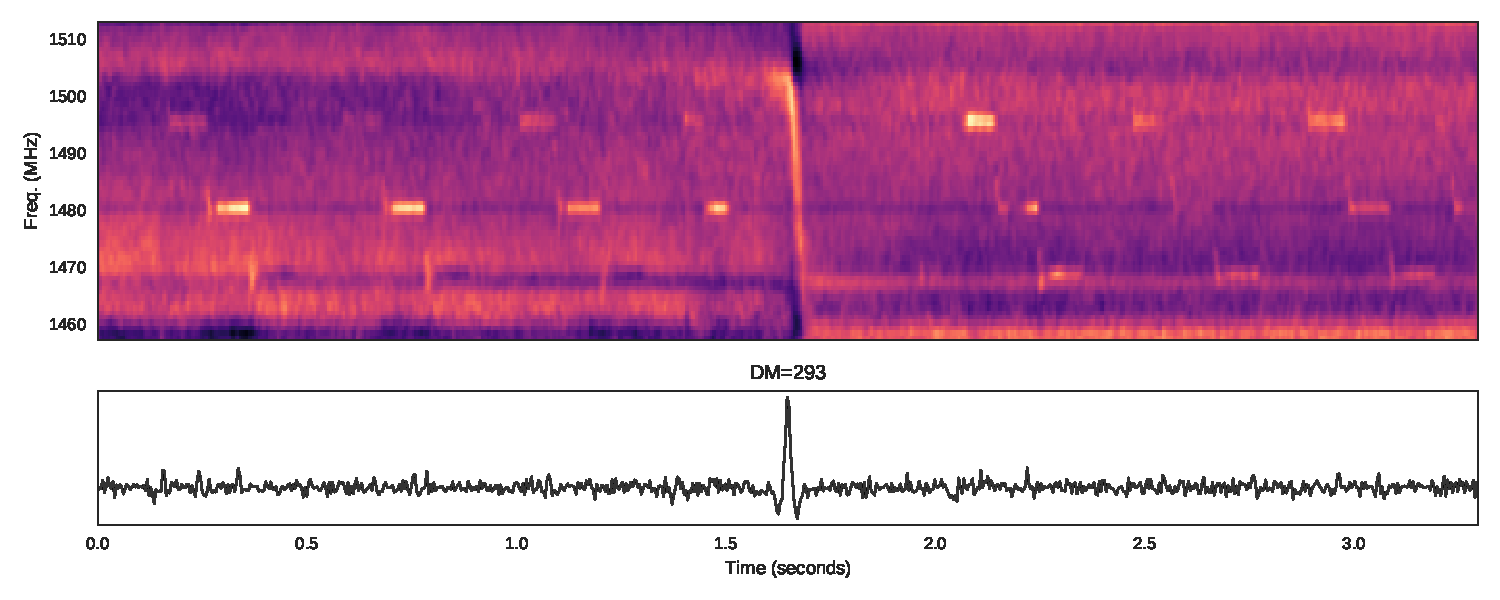
\includegraphics[width=1.0\linewidth]{figures/D20161204_buf23_Beam0_wide.pdf}
    \caption{Detected FRB-like event in beam 0 of ALFA. The characteristic dip
    before and after the event is due to zero-DM removal which is part of the
    ALFABURST RFI exciser. The strong, narrowband, repeating signal is due to a
    local RFI source.
    }
    \label{fig:beam0_dynamic_spec_wide}
\end{figure*}

\begin{figure*}
    \centering
    % watermark:terrestrial-frb-letter/notebooks/ALFABURST_events.ipynb
    \begin{subfigure}[t]{0.45\textwidth}
        \centering\captionsetup{width=.95\linewidth}
        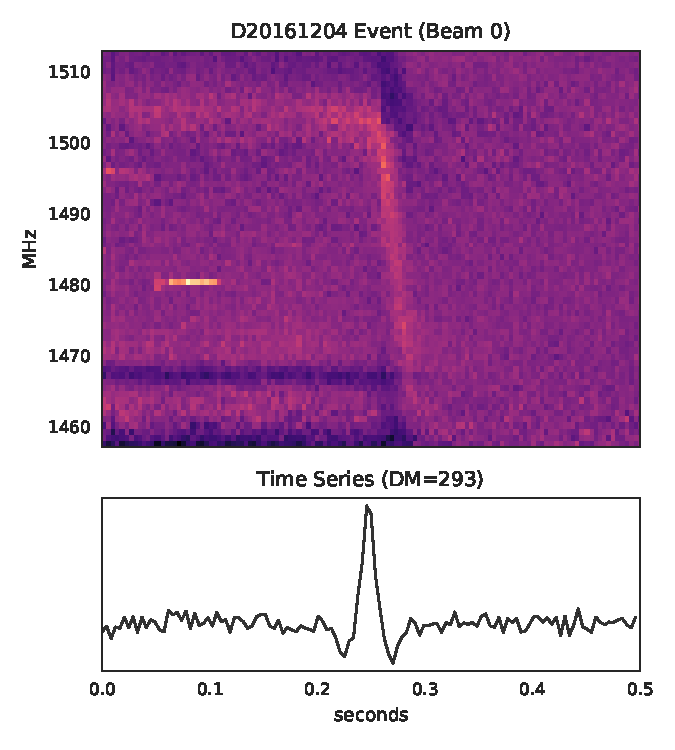
\includegraphics[width=1.0\textwidth]{figures/D20161204_buf23_Beam0.pdf}
        \caption{Detected FRB-like event in beam 0 of ALFA. The characteristic dip
        before and after the event is due to zero-DM removal which is part of the
        ALFABURST RFI exciser. The strong, narrowband source at 1480 MHz around 0.1
        s is due to a  local RFI source.  }
        \label{fig:beam0_dynamic_spec}
    \end{subfigure}
    % watermark:terrestrial-frb-letter/notebooks/ALFABURST_events.ipynb
    \begin{subfigure}[t]{0.45\textwidth}
        \centering\captionsetup{width=.95\linewidth}
        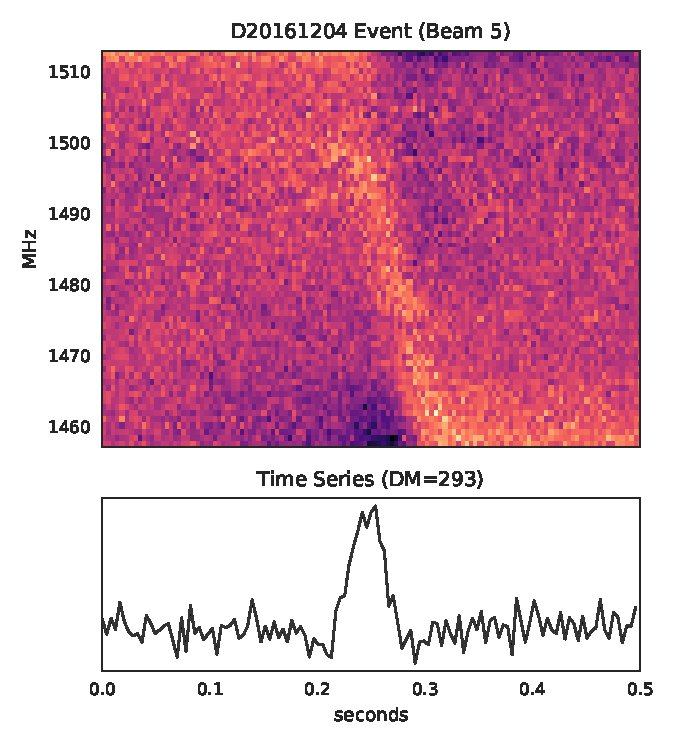
\includegraphics[width=1.0\textwidth]{figures/D20161204_buf4_Beam5.pdf}
        \caption{Detected FRB-like event in beam 5 of ALFA. The event width
        appears wider than the beam 0 event as the zero-DM dips are not as
        prominent.
        }
        \label{fig:beam5_dynamic_spec}
    \end{subfigure}
    \caption{
    Dynamic spectrum (top) and dedispersed time series (bottom) of an FRB-like
    event that was detected simultaneously in beam 0 and 5 of the ALFA receiver
    on December 4, 2016. The dynamic spectrum has been bandpass normalized.
    }
    \label{fig:dynamic_spec}
\end{figure*}

On initial inspection, this event looks like a promising new astrophysical
\gls{frb}. The flux density of the event can be computed with the radiometer
equation
%
$$
S = \textrm{SEFD} \frac{\textrm{SNR}}{\sqrt{D \; \Delta \tau \;
\Delta \nu}}\cM{,}
$$
%
using a \gls{sefd} of 3~Jy for the \gls{alfa} receiver. This results in a flux
density of $S = 66$~mJy from Beam 0, which would be \cM{a} lower flux than any
previously detected \gls{frb} \citep{2016PASA...33...45P}. This flux estimate is
a lower limit, as we are assuming the source was\cM{is?} at the centre of the beam. The
width is \cM{\sout{on the high end} large} for \glspl{frb} but \sout{still} within the range of those
previously reported.

We inspected all other events in the same time window as the Beam 0 event. An
event was found in Beam 5 only (Figure \ref{fig:beam5_dynamic_spec}). This pulse
lines up \sout{exactly in time} with the Beam 0 event \cM{in time exactly,} but the \gls{frb} was maximized
(\cM{$S/N=16$}) \cM{for \sout{with}} a DM of 829~pc~cm$^{-3}$ \cM{\sout{dedispersion}}. Upon further inspection and
testing different DMs \cM{\sout{for dedispersion}} we found that this event appeared to
narrow\cM{shrink?, decrease?} in width \cM{\sout{at}for} lower DM trials. We see\cM{saw, note?} that there was \gls{rfi} clipping in
this event which is known to introduce a bias, resulting in a maximized
\gls{snr} at a different DM trial. The beam 0 and beam 5 event are the same
event. \cM{consistency on caps for beam 0/Beam 0}

The beam 5 detection has a lower \gls{snr} than the beam 0 detection at \cM{a} DM trial
of 293~pc~cm$^{-3}$. This is \cM{\sout{still}} reasonable \cM{\sout{as} since} the beam 0 side-lobes overlap
with all the other beams, \cM{and\sout{does}} the beam 5 side-lobe\cM{s} overlap with the beam 0
primary beam. This would indicate that the sky source is somewhere between the
beam 0 and beam 5 pointing centres. And, the detection was from the edge of the
primary lobe or in the side-lobe of each beam.

The width of the dedispersed pulse in beam 5 appears wider, but this is likely
due to the lower \gls{snr} of the event having a smaller effect on the
spectrum normalization.

One can look at the immediate period before and after the pulse to see that
there are no similar events (Figure \ref{fig:dm_time}). \cM{you've moved from 'we' to 'one'} The event appears to be
isolated in time, with a fairly compact representation in DM-space (Figure
\ref{fig:dm_time_event}) similar to that of a single pulse from a \cM{\sout{higher
dispersed} `high DM' or `pulsar with a higher/larger DM'} pulsar such as \cM{PSR} B1859+03 (Figure \ref{fig:dm_time_B1859}). The event
would be detected with significant \gls{snr} at higher \gls{dm} trials due to
the \cM{\sout{wide} large} width of the pulse, but peaks at a \gls{dm} trial of 293~pc~cm$^{-3}$.

\begin{figure}
    \centering
    % watermark:terrestrial-frb-letter/notebooks/ALFABURST_events.ipynb
    \begin{subfigure}[t]{0.5\textwidth}
        \centering\captionsetup{width=.95\linewidth}
        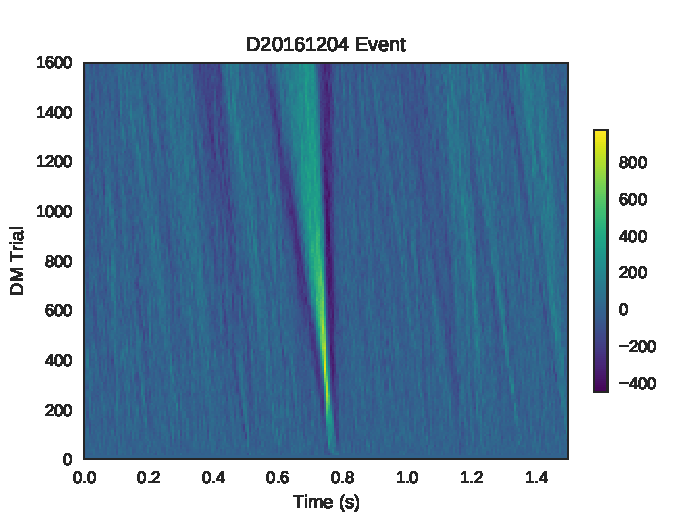
\includegraphics[width=1.0\textwidth]{figures/D20161204_dmtrials_buf23_Beam0.pdf}
        \caption{DM vs. time plot of for a 1.5 second window centred on the December
        4th event in beam 0. The SNR peaks at a DM of 293. There is a significant
        detection at larger DM trials due to the width of the pulse.
        }
        \label{fig:dm_time_event}
    \end{subfigure}
    % watermark:terrestrial-frb-letter/notebooks/ALFABURST_events.ipynb
    \begin{subfigure}[t]{0.5\textwidth}
        \centering\captionsetup{width=.95\linewidth}
        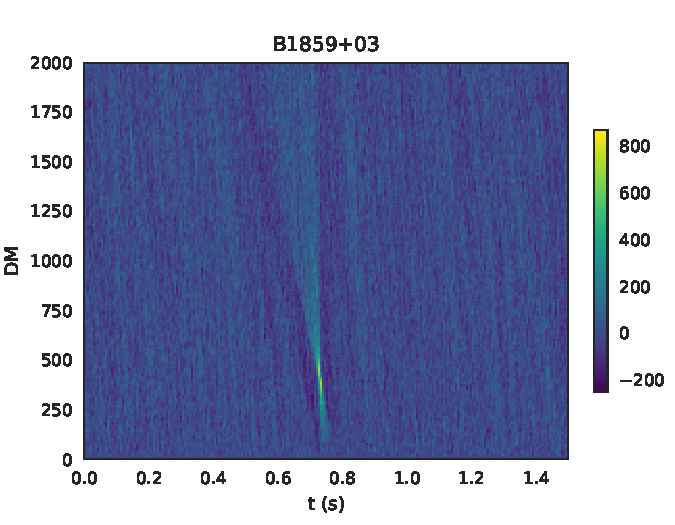
\includegraphics[width=1.0\textwidth]{figures/B1859_dmtrials.pdf}
        \caption{DM vs. time plot of a bright single pulse from B1859+03 which
        has a DM of 402~pc~cm$^{-3}$ and pulse width of 11~ms (W50).
        }
        \label{fig:dm_time_B1859}
    \end{subfigure}
    \caption{DM-space plot shows the characteristic butterfly pattern of the
    narrow-in-time, dispersed pulse detected by ALFABURST. A single pulse
    detection of B1859+03 is shown for reference.
    }
    \label{fig:dm_time}
\end{figure}

The Arecibo telescope logging data is reported locally in \cM{\sout{SCRAM} data?} packets which
provide pointing, frequency tuning, and receiver information at approximately
one second resolution. From these logs, \cM{this is just the info contained in the logs right? I'd just say the logs report/ed or something like that} the telescope was \cM{tenses!}pointed at a fixed Dec
(+15:11:28.34) and drifting in RA (event detected at RA=14:42:26.18), i.e. a
fixed (alt, az) pointing during the event. No known pulsar or RRAT with a similar
DM is nearby at this pointing.

We considered that the observing band could have been changed in that time.  We
have \cM{set up} the automated system to restart observations when the \gls{if}
frequency is changed.  During the time of the event, there was no change in the
\gls{if} during that time. \cM{perhaps too much detail}

The SCRAM logs \cM{\sout{do}} provide the first indication that this event is due to a local
source. Beyond the pointing and \gls{if}, the SCRAM logs report the position of
the receiver turret and \cM{\sout{if} report whether} \gls{alfa} is active. \gls{alfa} is at a position
angle of approximately $26.64^{\circ}$ in the turret, the system reported the
turret was at $206^{\circ}$. \gls{alfa} is not in, or even near the focus.  Our
commensal observation script checks if \gls{alfa} is active before we run
ALFABURST. This is a check on whether the analogue receiver chain is properly
setup for \gls{alfa}, which almost always means that \gls{alfa} is in the focus.
But, as we have found out, there are times when this is not true. \cM{it might be worth seeing if you can shorten the above paragraph quite a bit.}

The SCRAM logs do not report the active project or observing schedule. During
the time of the event it appears that no receiver was in use, otherwise,
\gls{alfa} would not have been active, and we see that \gls{alfa} was
deactivated approximately 20 minutes after the event when a new observation
began.  Looking at the observation schedule for the morning of December 4,
project
P3080\footnote{http://www.naic.edu/vscience/schedule/tpfiles/MichillitagP3080tp.pdf}
was using \gls{alfa} to perform an \gls{frb} survey of the Virgo cluster until
09:00 local time.  After 09:00 local time Project
R3037\footnote{http://www.naic.edu/vscience/schedule/tpfiles/TaylortagR3037tp.pdf}
was scheduled, this is an S-Band RADAR observation. \cM{it might be worth seeing if you can shorten the above section about the receiver position/activity quite a bit.}

\cM{\sout{Looking at}} the average bandpass of beam 0 and 5 during the time of the event, \cM{\sout{we
see} shows?} that the shape and system noise appear different to what is expected during
typical observations (Figure \ref{fig:bandpass_response}).  The detection band
of \gls{alfa} was chosen because it is the most sensitive region of the band,
and relatively flat. But during the event, there is a noticeable shape and slant
to the bandpass which is different than the typical bandpass.  Beam 0 and 5
bandpasses \cM{\sout{look} appear similar and have overlapping narrow-band RFI features \sout{related in elements of their bandpass shape, and the narrow-band
features due to the short, bright \gls{rfi} events that occur during the
recorded time window.}} The system noise appears to be higher during the event,
which leads to \cM{\sout{the} smoother bandpasses \sout{appearing smoother} than what is \sout{the} typical \sout{bandpass}}.  In
the detection pipeline the data is normalized, \sout{so} which removes all absolute scaling \sout{is
removed} in the process. This indicates that the \gls{sefd} is too low in our
flux calibration. This increase \cM{in} system noise is due to the change in turret
position, and the \gls{alfa} feed picking up reflections from other equipment in
the dome, and the dome as a warm source. \cM{a bit clumsy}

% watermark:terrestrial-frb-letter/notebooks/ALFABURST_events.ipynb
\begin{figure}
    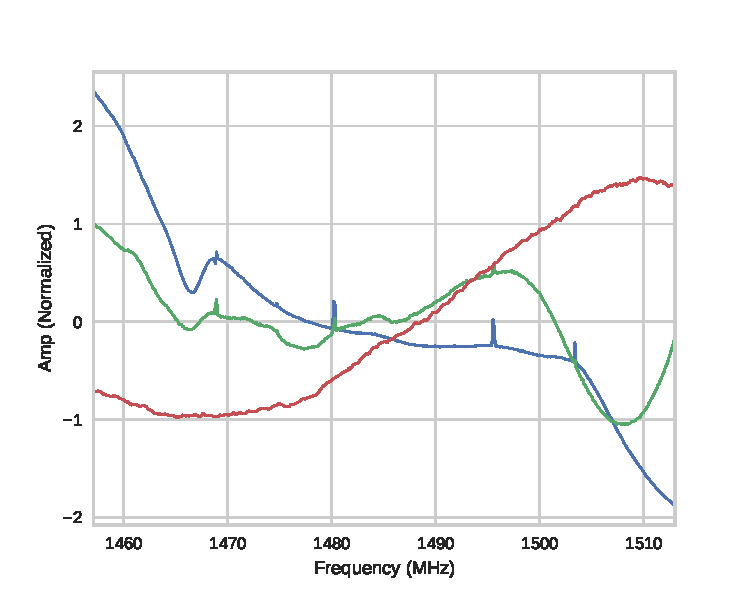
\includegraphics[width=1.0\linewidth]{figures/bandpass_response.pdf}
    \caption{Average bandpass response during the December 4, 2016 event for beam
    0 (green) and beam 5 (blue). A typical bandpass (red) is plotted for
    reference. These bandpasses have been normalized in the detection pipeline.
    }
    \label{fig:bandpass_response}
\end{figure}

We then looked at previously recorded events close in time to the event.
Approximately 80 seconds earlier another window was recorded which has large
structures across the band (Figure \ref{fig:beam0_dynamic_spec_80s}). Though not
as narrow in time as the event, they appear related to the same phenomenon.

The DM$-$time plot (Figure \ref{fig:beam0_dmtrials_80s}) shows that much of the
structure would be detected as dispersed pulses.  In particular, the structure
around 4 seconds would be detected as a wide-in-time, highly dispersed pulse.
And the structure immediately proceeding it would be detected as a negative\cM{ly}
dispersed pulse.  We do not detect these as pulses because we have limited our
search space to narrow-in-time width pulses and positive \glspl{dm}. Our choice
of search space is reasonable for the type of events we wish to detect given
limited computing resources. But, there are practical advantages to searching
negative \glspl{dm} and wider-in-time pulse widths. We expect astrophysical
pulses to have positive \glspl{dm}. But, system variation and \gls{rfi} can
produce signals which result in positive and negative \gls{dm} detections.  A
statistical measure can be \cM{\sout{made} computed/constructed} in any time window to differentiate times of
significant, but low-level \gls{rfi} or system variation from actual
astrophysical pulses. Testing out to larger pulse widths is computationally
cheap as the time window is decimated, reducing the memory usage. A full sampling
of larger pulse widths or negative \gls{dm} trials \cM{\sout{like} similar to?} the positive \gls{dm}
trials is not necessary. Only a subset can be computed to provide \sout{a} useful
information on the stability of the system and \cM{the} \gls{rfi} environment.

\begin{figure*}
    \centering
    % watermark:terrestrial-frb-letter/notebooks/ALFABURST_events.ipynb
    \begin{subfigure}[t]{1.0\textwidth}
        \centering\captionsetup{width=.95\linewidth}
        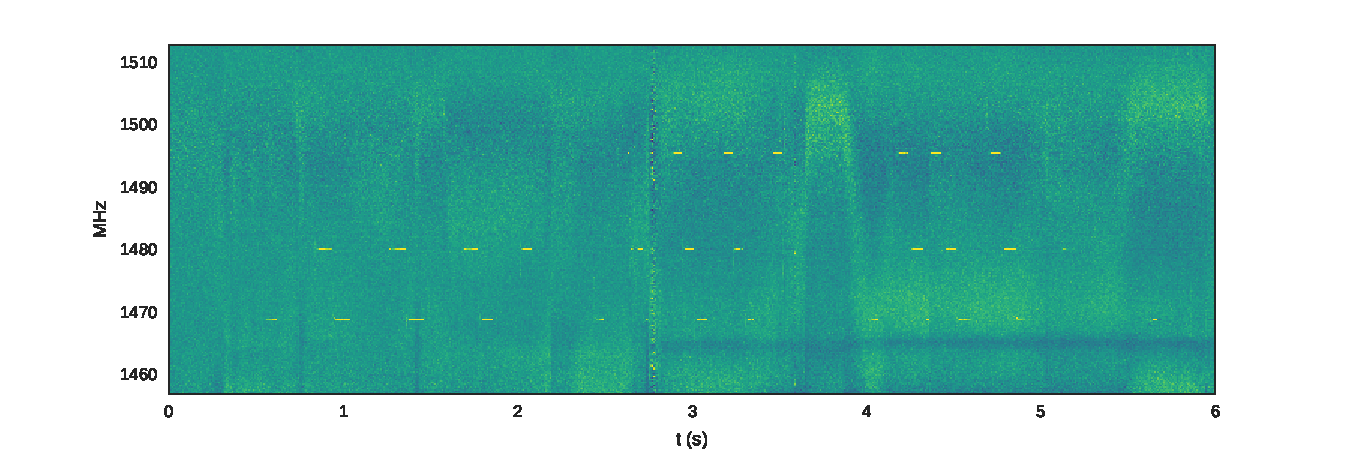
\includegraphics[width=1.0\textwidth]{figures/D20161204_spect_buf21_Beam0.pdf}
        \caption{Dynamic spectrum shows frequency evolution of the bandpass as a
        function of time with structures similar to the D20161204 event.
        }
        \label{fig:beam0_dynamic_spec_80s}
    \end{subfigure}
    % watermark:terrestrial-frb-letter/notebooks/ALFABURST_events.ipynb
    \begin{subfigure}[t]{1.0\textwidth}
        \centering\captionsetup{width=.95\linewidth}
        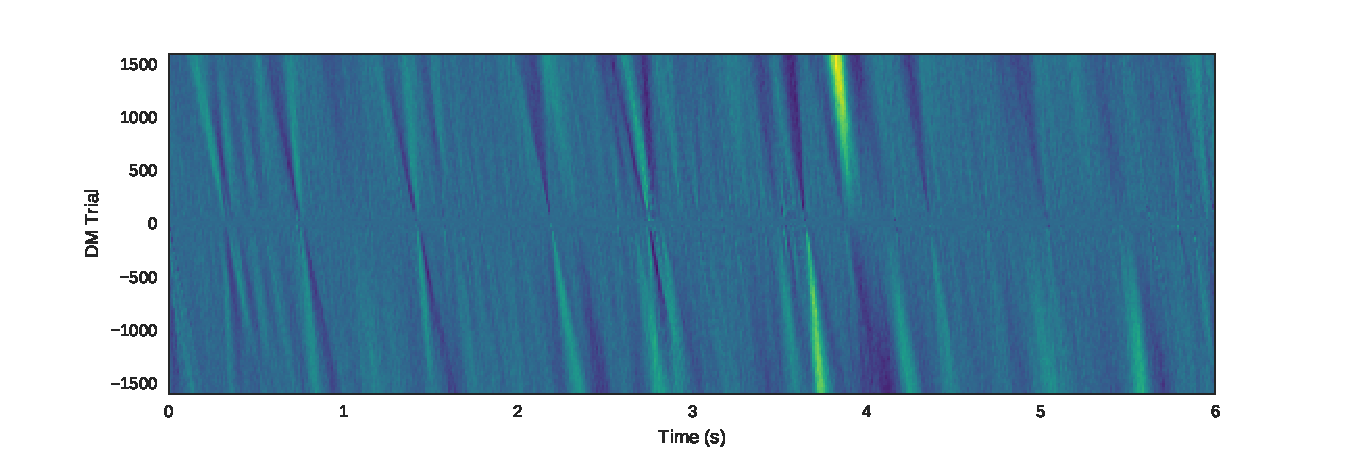
\includegraphics[width=1.0\textwidth]{figures/D20161204_dmtrials_buf21_Beam0.pdf}
        \caption{DM trials from -1600 to 1600 show that there would be both
        positive and negative pulse detections during this time window.
        }
        \label{fig:beam0_dmtrials_80s}
    \end{subfigure}
    \caption{Dynamic spectrum (top) and DM-time plot (bottom) of 6 seconds from
    beam 0 approximately 80 seconds before the D20161204 event.
    }
    \label{fig:beamo0_80s}
\end{figure*}

The narrow-in-frequency, periodic RFI at 1468, 1480, 1496,
1504~MHz is not usually seen in this band. In the high time and frequency
resolution view these short pulses in 12.5~MHz steps have a characteristic
dampened harmonic oscillation due to frequency locking with a \gls{pll} (Figure
\ref{fig:pll_spectrum}). With help from the Arecibo Observatory staff, this has
been identified as instrumentational \gls{rfi} from an instrument that is
routinely used to monitor the local \gls{rfi} environment.

% watermark:terrestrial-frb-letter/notebooks/ALFABURST_events.ipynb
\begin{figure}
    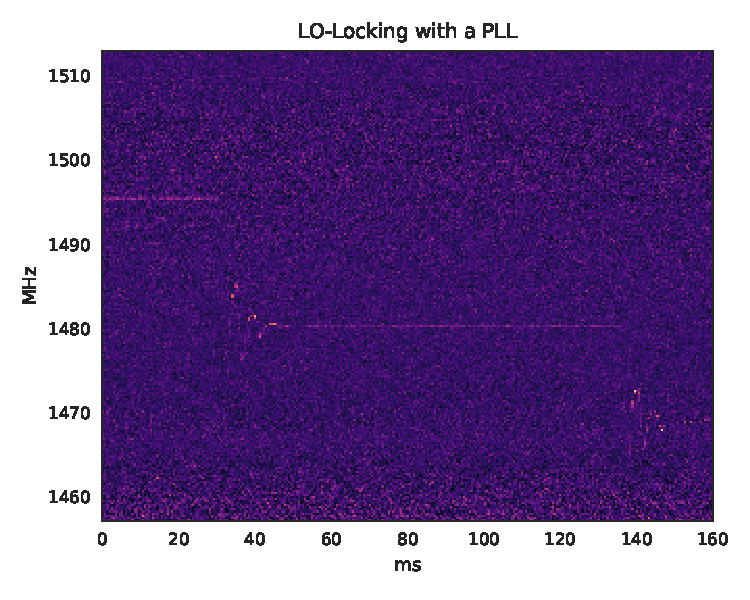
\includegraphics[width=1.0\linewidth]{figures/pll_spectrum.pdf}
    \caption{Dynamic spectrum when a local oscillator in the receiver dome is
    being locked with a phase-locked loop circuit. This LO is not related to
    the receiver analogue mixing chain, but rather it is associated with RFI
    monitoring equipment.
    }
    \label{fig:pll_spectrum}
\end{figure}

The cause of this FRB-like event was \cM{likely?} due to \cM{\sout{some} a} component of the analogue chain
saturating and \cM{\sout{going to} reaching? evolving to?} a non-linear state.  An \gls{rfi} monitoring program was
\sout{being} run on an instrument not included in the telescope SCRAM data. This
instrument introduced the narrowband \gls{rfi} due to changing of a \gls{lo}. \cM{if you don't remove IF from before, it's probably worth being consistent across.}
The \gls{alfa} receiver was out of the main focus, likely picking up reflections
from the dome, leading to an increase in the system temperature.  This increase
caused some part of the analogue chain, likely an amplifier, to operate beyond
it's linear response region and produce broadband oscillations. \cM{somewhat repetitive, you can probably shorten.} With high
certainty, we can classify this as a local event which created the appearance of
an \gls{frb}.  In isolation, and \cM{taking into account} the one-off, transient nature of FRBs, \sout{make} the
initial Beam 0 detection \cM{looks} \cM{seems?} very reasonable \cM{the detection is reasonable. You have to say something like seems real or astrophysical}. It is only with an extended study
of the meta-data, earlier-in-time evolution of the band, and use of multiple
beams to confirm that this is \cM{\sout{indeed}} not an FRB of astronomical origin.

\section{Low-SNR False-Positive Detections}
\label{sec:low_snr}

As the automated search pipeline is \cM{set up} to do an extensive search in \gls{dm}
trails, pulse width, and starting time it is reasonable to expect a large number
of low-SNR false-detections.  \gls{frb} surveys tend to have a significant
minimum \gls{snr} cut-off (6$-$10) due to the large number of false-positive
detections at low \glspl{snr}.  In the ALFABURST and ARTEMIS
\citep{2015MNRAS.452.1254K} surveys the minimum SNR cut-off is set to 10.

Low-SNR detections are regularly detected even with high minimum SNR cut-off.
For example, on July 30, 2015 an apparently 10-sigma event with a DM of
1370~pc~cm$^{-3}$ was detected (Figure \ref{fig:D20150730}). The pulse can
barely be seen in the spectrogram, but in the DM-space plot there is a compact
peak centred at a DM of 1370~pc~cm$^{-3}$. This event is \cM{suspicious} because the
D20161204 event discussed earlier only has a slightly higher SNR but is visible
in the spectrogram. The resolution is that the \cM{\sout{actual}real} SNR of this event is
approximately 6, while a the reported value of 10 \sout{The SNR of 10 reported} is based on a longer running average
computed in the automated pipeline. \sout{Looking only} \cM{Locally} in time there is an
increase in system noise, leading to a reduced SNR. The increase \cM{in} system noise
is \cM{caused} \sout{because the} \cM{by the} receiver turret \sout{began} rotating \sout{in this period} while the ALFA
receiver was still active. \cM{or shorten in a similar way}

% watermark:terrestrial-frb-letter/notebooks/ALFABURST_events.ipynb
\begin{figure}
    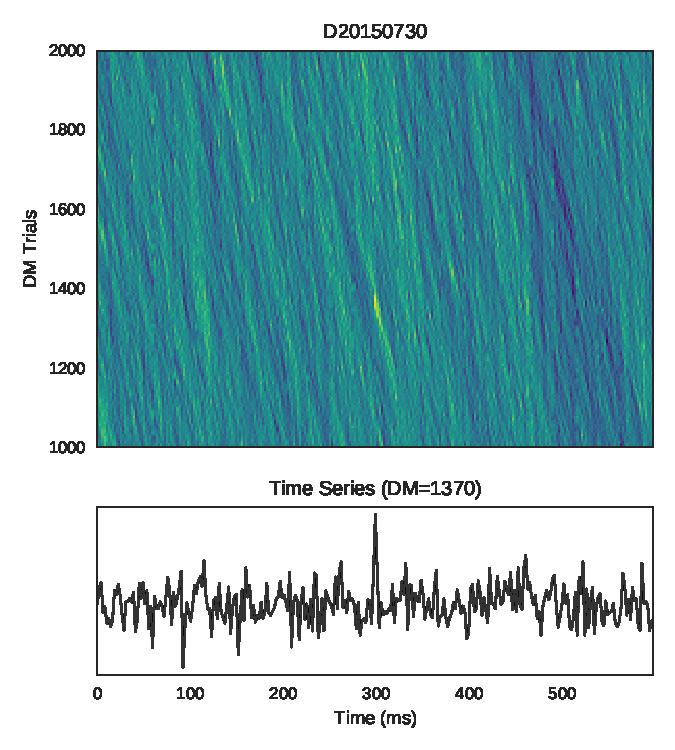
\includegraphics[width=1.0\linewidth]{figures/D20150730_buf23_Beam6_dmtrial.pdf}
    \caption{DM-space plot and time series of a high DM event with reported SNR
    above 10-sigma on July 30, 2015. After re-analysis and review of the
    telescope metadata \cM{or meta-data, consistency} it was determined that this event was due to local system
    noise.
    }
    \label{fig:D20150730}
\end{figure}

The reported detection of a pulse from FRB121102 with APERTIF \citep{atel10693}
\sout{was at} \cM{had an} SNR$\approx 4$. In a blind survey across different sky positions and DM
trials this would not be a significant detection. But, the sky position and
SNR-maximized DM of the repeater \cM{I guess repeater is ok. But maybe repeating FRB is better} is known, thus a lower SNR detection may be
reasonable to report.  We require a large \gls{snr} to validate a detection.  As
the parameter space (DM trials, pulse width range) and number of observations
grow we \sout{should} expect to see an increase in the number of high-\gls{snr},
false-poisitive events.

\section{Detected RADAR Event with ARTEMIS}
\label{sec:LOFAR_RADAR}

ARTEMIS \citep{2015MNRAS.452.1254K} is \cM{an \gls{frb} search
survey, similar to ALFABURST}, run \cM{on?\sout{at}} the LOFAR-UK station at \cM{the} Chilbolton Observatory. The ARTEMIS survey uses a similar fractional bandwidth ($\sim 0.04$) to \sout{the} ALFABURST \sout{survey}, but \cM{is}
centred \cM{at $\sim$?} 145~MHz. \cM{\sout{This survey is \cM{set up, designed?} to have}} \cM{In this survey} known pulsars regularly
transit the fixed in local coordinate beams. \cM{rather the beams that are fixed in local coordinates?} \cM{and} single pulses are routinely
\cM{\sout{detected} observed}. Occasionally, \gls{rfi} events are detected by the automated pipeline.
A particularly interesting event \sout{was detected} \cM{for} which \sout{had a} \cM{the \gls{snr} was maximized} at a  
\sout{with a} \gls{dm}$= 85$~pc~cm$^{-3}$ is shown in Figure \ref{fig:lofar_dynamic}.
The narrow-in-time pulse can be seen in the dynamic spectrum at frequencies
above 146 MHz, but \sout{is} not \sout{apparent} at lower frequencies. \cM{where it could be buried by narrow band \gls{rfi}?} \sout{As there is significant
narrow band \gls{rfi} below 146 MHz it could be that the pulse is buried. } The
dedispered time series shows a strong\cM{?clear?} detection of a pulse of approximately
20~ms in width.

% watermark:terrestrial-frb-letter/notebooks/LOFAR_RADAR.ipynb
\begin{figure}
    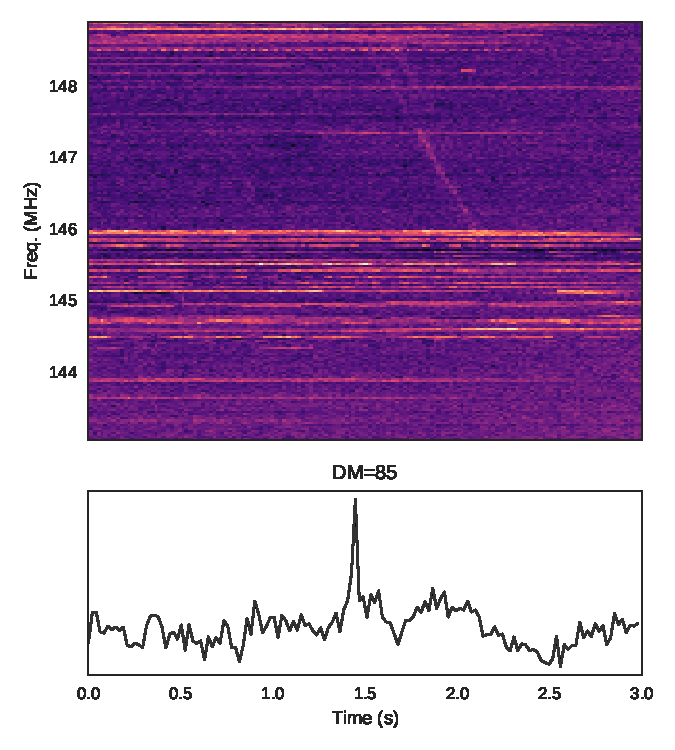
\includegraphics[width=1.0\linewidth]{figures/LOFAR_dynamic.pdf}
    \caption{A dispersed pulse detected by the automated ARTEMIS search
    pipeline. The dispersed pulse only appears over a narrow band of just over
    1~MHz.
    }
    \label{fig:lofar_dynamic}
\end{figure}

The celestial pointing of the beam \cM{just 'The celestial pointing' or just 'the beam pointing'?} during the time of the event is not
associated with any known pulsar or RRAT at a DM\cM{$\sim$ \sout{around}} 85~pc~cm$^{-3}$. This \sout{is}
DM is low compared to reported \gls{frb} detections.
% TODO: pointing, SNR, maximized DM and time decimation, NE2001 model for
% distance

Plotting the event in \cM{\sout{a}} DM-space across the ARTEMIS DM range
($0-320$~pc~cm$^{-3}$\cM{\sout{) (},} Figure \ref{fig:lofar_dm_time}) shows a strong, compact
detection \cM{\sout{which we would expect to see} as expected} of a dispersed pulse during a time of
minimal \gls{rfi}.

% watermark:terrestrial-frb-letter/notebooks/LOFAR_RADAR.ipynb
\begin{figure}
    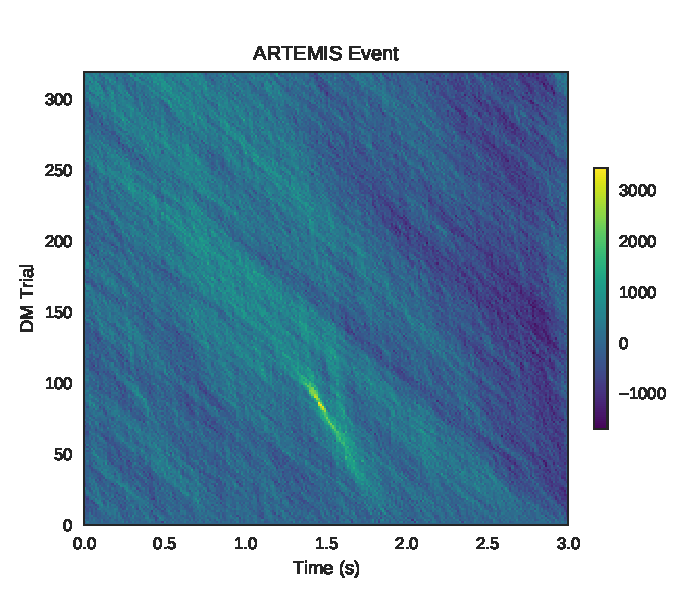
\includegraphics[width=1.0\linewidth]{figures/LOFAR_dm_time.pdf}
    \caption{DM-space plot of the event shows a strong, compact detection around
    a DM of 85~pc~cm$^{-3}$ with no other apparent events during at the time.
    }
    \label{fig:lofar_dm_time}
\end{figure}

Since the pulse is \sout{only} apparent in \cM{only} part of the band, we became suspicious of its
origin. \cM{Tenses. Strange story telling style. I'd say Since blah blah it's origin is suspicious/unclear} 
It could be that the pulse is broadband \sout{but} \cM{and only} the brightest component is
\sout{only} seen in the 146-147~MHz region. Or, it could be a band-limited pulse.  The
search pipeline \cM{ARTEMIS instead? Been a while since it's name has been mentioned}, like ALFABURST and many other search pipelines, decimates the
dynamic spectrum in time to search \sout{for} over a range of pulse widths. \cM{\sout{In the case
of t}T}he \cM{\gls{snr} of the} event shown in Figure \ref{fig:lofar_dynamic} \cM{is} maximized 
\cM{\sout{occurred with a}} \cM{for a} time decimation factor of 64\sout{,}\cM{. With a \sout{the} native resolution \sout{is} of} $327.68
\mu s$, \cM{this results} \sout{resulting} in a decimated time resolution of 20~ms. \sout{By  p}Plotting the event
at a higher time resolution\sout{s} (Figure \ref{fig:lofar_dynamic_high}) we \sout{can} see
\sout{there is} a distinct repeating pattern in time, \cM{\sout{not} previously not visible \sout{apparent}}. This is a
linearly frequency modulated signal used for pulse compression in RADAR.

% Linear Frequency Modulated Pulse Waveforms
% https://en.wikipedia.org/wiki/Pulse_compression
% http://www.radartutorial.eu/02.basics/Stepped%20Chirp%20Radar.en.html
% google: radar chirp l band, radar chirp quadratic, stepped chirp l band
% stepped chirp waveform
In RADAR observations\cM{,} the bandwidth of the transmitter provides information on
the range and direction of a target. A narrow band RADAR transmitter can be used
to approximate a larger bandwidth by modulating the frequency of the transmitted
pulse. The narrow band (in frequency) pulse is stepped in frequency across a
transmission band. Between each step the pulse is not transmitted, resulting in
the gaps in time between pulses in Figure \ref{fig:lofar_dynamic_high}. Linear
frequency modulation is the most typical form of chirp compression, but
non-linear methods are also used. A windowing function can be applied to the
pulse which can produce quadratic frequency modulations.  There are a number of
allocated usages in this band which could be the source of \cM{the observed \sout{this}} RADAR pulse
\citep{ofcom2017}. RADAR is also \sout{known to be} used from UHF to C-band, all \cM{covering a wide range of? instead of all}
frequencies \cM{at} which \gls{frb} surveys operate. As RADAR is used for commercial and
military \cM{purposes}, most of these signal specifications and modulations are proprietary.
We as astronomers likely will not have access to this type of information.  This
adds the extra step of verifying a source is astrophysical when reporting an
\gls{frb}. \cM{last two sentences are a bit clumsy}

% watermark:terrestrial-frb-letter/notebooks/LOFAR_RADAR.ipynb
\begin{figure}
    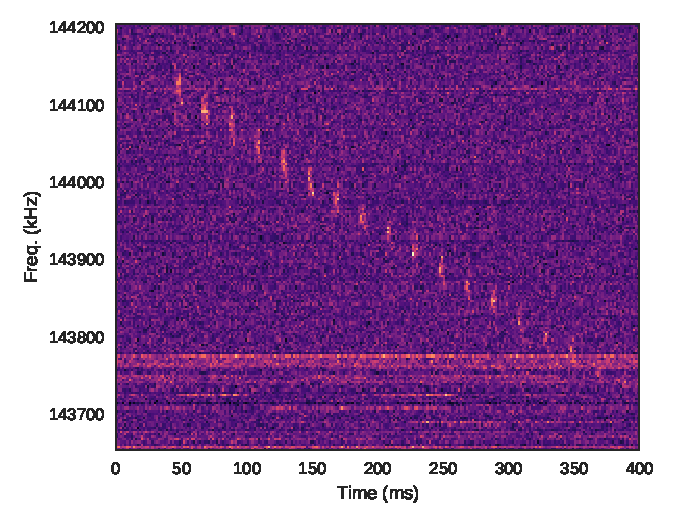
\includegraphics[width=1.0\linewidth]{figures/LOFAR_dynamic_high_res.pdf}
    \caption{A zoomed in view of the event in Figure \ref{fig:lofar_dynamic} at
    high time and frequency resolution shows the distinct pattern of a linearly frequency
    modulated RADAR pulse.
    }
    \label{fig:lofar_dynamic_high}
\end{figure}

As the RADAR signal is a dispersed pulse we \sout{would} expect to detect such signals
with \gls{frb} pipelines.  Verification of this event \cM{is?\sout{was}} \cM{straightforward} \cM{\sout{by} when}
examining the high-time and frequency resolution data \cM{that reveal the} \sout{to see the} pulsed nature
of the event.  The frequency allocation and the use of standard RADAR techniques
across the radio band \cM{\sout{is} are \sout{a} clear indicators} of the origin of this event.  

\sout{A
challenge comes in the} verification \cM{becomes challenging when} \sout{and automated signaling if} the desire is to
run the system in real-time with immediate follow-up with additional telescopes.
Expert knowledge in the instrument, radio signals and visual acuity were
necessary to identify this rare RADAR event.  Automating this process is
difficult, so if we desire an automated VOevent trigger, we should expect a
number of false-positive triggers. \cM{shorten}

\section{XAO Repeating Event}
\label{sec:xao_event}

The 25-m Nanshan Telescope at \gls{xao} is currently running an FRB survey. The
survey covers over 300~MHz at L-band, sampling at $64 \; \mu s$ resolution. On
November 18, 2016 hundreds of bright, dispersed pulses were detected \sout{with the
system}. The\sout{se} pulses varied in SNR, but had the same SNR-maximized DM of
531.8~pc~cm$^{-3}$. The pulses show a distinct double peak (\cM{each peak?} $\sim 2$~ms \cM{wide})
separated by $\sim 3$~ms (Figure \ref{fig:xao_dynamic}). The pulse \cM{shows up in only?} \sout{is only
apparent in a} about a quarter of the band.

% watermark:/home/griffin/data/XAO/coadd_pulses.ipynb
\begin{figure}
    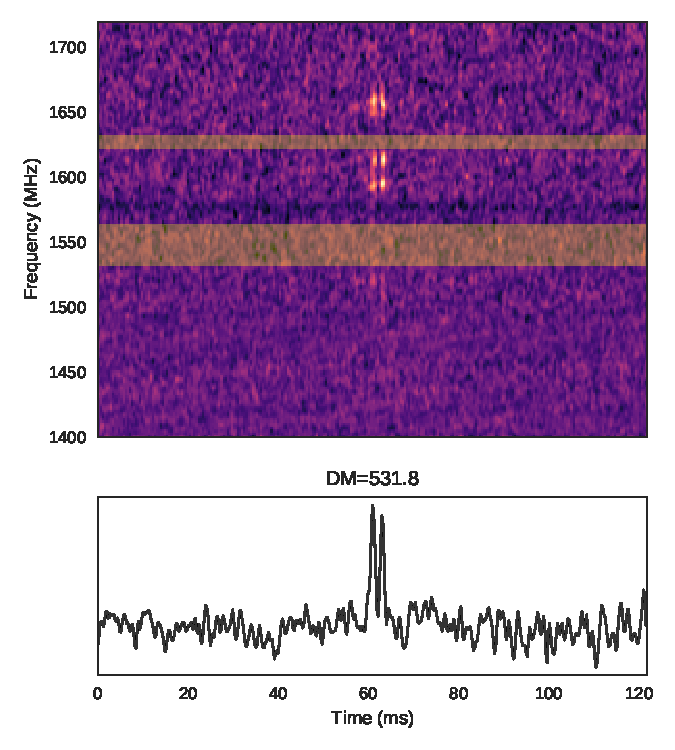
\includegraphics[width=1.0\linewidth]{figures/XAO_pulse_dynamic.pdf}
    \caption{Example of a detected pulse with the Nanshan Radio Telescope at XAO
    which is SNR maximized at a dedispersion of $531.8$~pc~cm$^{-3}$. Hundreds
    of such pulses were detected over a period of a few days. The orange bars
    represent regions that have had significant constant-in-time RFI removed.
    }
    \label{fig:xao_dynamic}
\end{figure}

\sout{No pointing is reported here as }The pulses were seen at different pointings
across the sky. Most were detected at a low altitude pointing angle, but some
were detected \sout{with the dish pointed }close to zenith.

A periodicity search \cM{\sout{was run on the observation,} revealed} a periodicity of $\sim 1.7$ \cM{units? \sout{was
found}}, but the residuals were significantly higher than that of \sout{residuals from} a
typical pulsar periodicity search. \cM{This along with the pointing variability
rules out a pulsar, or an astronomical source in general.}

\cM{A thorough search of possible local sources, such as new equipment, vehicles,
and aircraft was preformed. No obvious candidate was found. - I would move these 2 sentences to the end of the paragraph.} A dispersion
relation parameter estimation found that pulses deviate from a $\nu^{-2}$
relation by $1.5 \sigma$. \cM{Figure \ref{fig:xao_summed} shows the sum of the dedispersed (using DM
531.8~pc~cm$^{-3}$) phase-aligned pulses.  \sout{This can be seen by aligning the pulses, and summing
them together (Figure \ref{fig:xao_summed}). $\nu^{-2}$ dedispersion} The addition produces an S-shaped broadband pulse with \cM{frequency} structure that is not
seen in the individual pulses.} \sout{There is also \cM{\sout{apparent}clear? - think apparent is overused} regular, narrow-band
frequency modulation in the pulse structure.} The \sout{is broad-band} structure is due to
non-linearly frequency modulation, \cM{used in chirped RADAR systems, which is different from the linear modulation observed in Sec. blah.}
\sout{This type of modulation is used in chirped
RADAR systems, though it is not as common as linear frequency modulation.} \cM{maybe I've not done the best at shortening this, main idea is to shorten.}

% watermark:/home/griffin/data/XAO/coadd_pulses.ipynb
\begin{figure}
    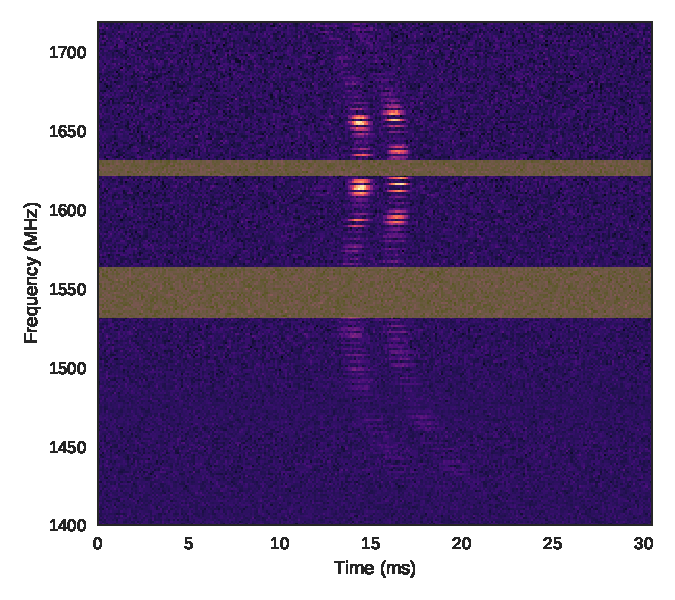
\includegraphics[width=1.0\linewidth]{figures/XAO_summed_dynamic.pdf}
    \caption{The dynamic spectrum of 182 high-SNR pulses detected with the
    Nanshan Radio Telescope summed together.  The low-level, non-linear
    frequency modulation can be seen across the band. The orange bars represent
    regions that have had significant constant-in-time RFI removed.
    }
    \label{fig:xao_summed}
\end{figure}

\cM{I would add your previous sentences about ruling out astro sources and checking equip here. I guess your order comes from the chronology of the investigation.}
Detection of multiple pulses at different beam pointings indicates the source
may be directly illuminating the feed. The source is likely not due to system
electronics because of the complex frequency modulation\cM{\sout{. The likely source of
these pulses is}but rather due to} a local transmitter. Had only a single pulse been detected with
the telescope, for example if the source was weaker, or the telescope was only
sensitive to the highest SNR event, it would be difficult to show that the event
was due to RFI. Multiple reported \glspl{frb} do not cover the entire observing
band. This has been \cM{big mix of tenses} explained by various astronomical effects (scintillation,
plasma lenses). In this case, it would be reasonable to report a single pulse as
an \gls{frb}. The Nanshan L-band receiver is a single pixel system. It could be
that a multi-beam system such as the Parkes Multi-beam or ALFA would detection
these events in many of the beams. In that case, the detections could be
classified as local \gls{rfi}.

\cM{I would put the next paragraph(s) before doing the 'warning' of had only a single pulse been detected, since it forms part of the non-lin modulation discussion/analysis.}
The non-linear modulation scheme can produce a range of apparent SNR-maximized
events depending on the observing band compared to the pulse transmission band
(Figure \ref{fig:xao_simulated_dm}).  A simple model of the pulse can be
produced by using a logistic function which covers a bandwidth from
$\nu_{\textrm{p,0}} = 1350$~MHz to $\nu_{\textrm{p,1}} = 1750$~MHz (Figure
\ref{fig:xao_simulation_diagram}). The time duration of the pulse $\Delta
t_{\textrm{pulse}}$ is fixed such that central frequency range of the pulse has
an SNR-maximized DM of approximately 530~pc~cm$^{-3}$. The pulse \cM{is} given a width
\cM{($\Delta t_{\textrm{width}}$)} by convolving the logistic function with a 3~ms wide
Gaussian. The pulse is set to unity amplitude across the extent \cM{of the band?}.

% figures/simulation_digram.odg
\begin{figure}
    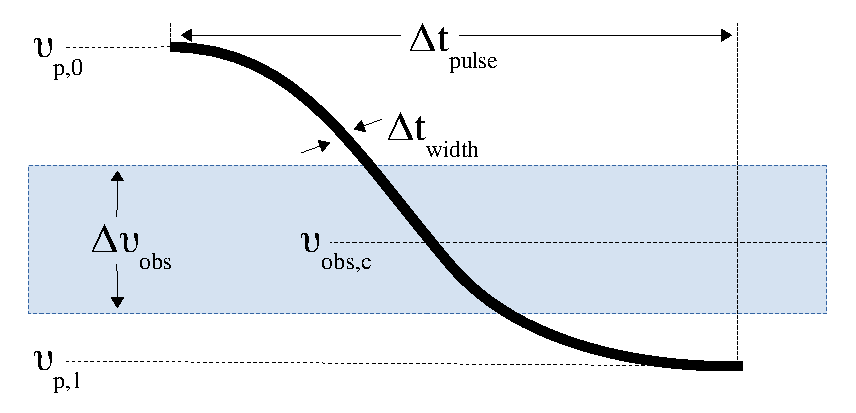
\includegraphics[width=1.0\linewidth]{figures/simulation_diagram.pdf}
    \caption{Non-linearly modulated pulse and receiver model used to simulate
    the response and SNR-maximized DM fit to a pulse similar to the one detected
    at XAO.
    }
    \label{fig:xao_simulation_diagram}
\end{figure}

A receiver model is used to simulate the observation. This model is
parameterized by central observing frequency $\nu_{\textrm{obs,c}}$, bandwidth
$\Delta \nu_{\textrm{obs}}$, number of observing frequency channels
$n_{\textrm{freqs}}$, and per channel noise $\sigma_{\textrm{chan}}$. The
bandpass is modelled as a Gaussian.

% watermark:/home/griffin/data/XAO/Non-Linear-Pulse-Simulation.ipynb
\begin{figure}
    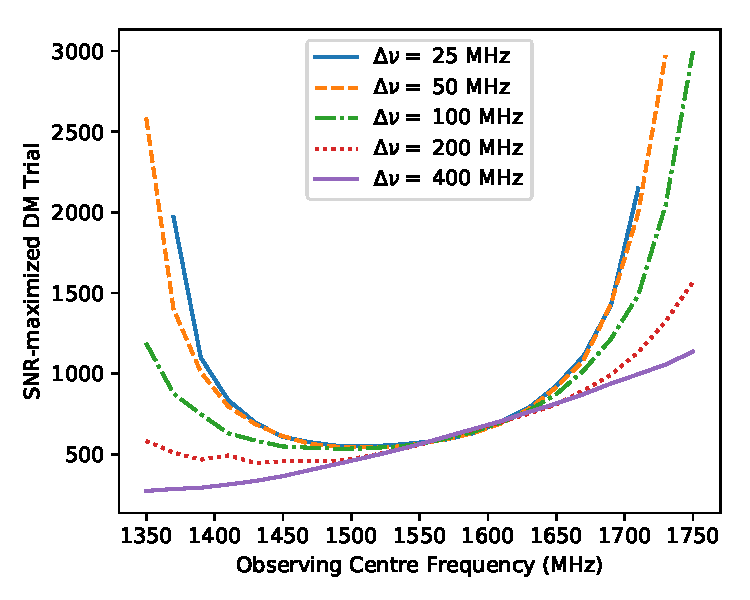
\includegraphics[width=1.0\linewidth]{figures/simulatedRADARdm.pdf}
    \caption{SNR-maximized DM trials for a simulation of the XAO non-linearly
    modulated pulse over a range of central observing frequencies, and receiver
    bandwidths.
    }
    \label{fig:xao_simulated_dm}
\end{figure}

Detection of the pulse is simulated across a range of central observing
frequencies and receiver bandwidths. The SNR-maximized DM is \sout{then} determined by
performing a trial DM search from 0 to 4000~pc~cm$^{-3}$ in integer increments.
For all bandwidths, when the central observing frequency is near the centre of
the pulse the apparent DM of $\sim530$~pc~cm$^{-3}$ maximizes the detection
SNR. However, when the central observing frequency is shifted relative to the
pulse centre frequency a range of SNR-maximized DM's are reported, depending on
the receiver bandwidth. This non-linearly modulated pulse will appear very
similar to an FRB detection at a receiver-dependent DM trial value. The top and
bottom of the pulse will likely appear as RFI due to the curve of the pulse \cM{this is a bit confusing, you mean due to the shape of the logistic function or the curve of the pulse in time-freq space}.

The source was only detected over the course of a day, and the origin remains
unknown.  Observations a XAO continue, with an interest in observing in November
2017 to see if the signal returns on an annual schedule. \cM{whoops that's already gone by... any thoughts on what they found?}

\section{Previously Reported FRBs}
\label{sec:previous_frbs}

Given that systematic effects and \gls{rfi} can produce apparent \glspl{frb} it
is useful to look back at previously reported \glspl{frb} that don't fit the
ideal broad-band, single component structure that detection pipelines are
optimized for.

% every FRB paper starts out with a definition, make that the fundamental
% checklist. which FRBs fail or succeed?
% TODO: what are questions that can be answered? aristotlian catagorization
% Check list of items:
%   broadband? scattered? multiple components?
%   multi-beam system
%   variation from the average bandpass
%   pointing? near the horizon?
%   repeats? repeats at different pointings?
%   resolved in time and frequency?
%   dispersion index fit
% Table of reported FRBs and events from this paper

% TODO: references
\begin{table*}
\centering
\begin{tabular}{ r l l r r }
Name      & Telescope & DM (pc~cm$^{-3}$)& Width (ms) & SNR  \\
\hline
FRB010125 & Parkes  & $790 \pm 3$        &  9.4 	&	17   \\ 
FRB010621 & Parkes  & $745 \pm 10$       &  7		&	16.3 \\
FRB010724 & Parkes  & $375$              &  5		&	23   \\ 
FRB090625 & Parkes  & $899.55 \pm 0.01$  &  1.92	&	30   \\ 
FRB110220 & Parkes  & $944.38 \pm 0.05$  &  5.6		&	49   \\ 
FRB110523 & GBT     & $623.3 \pm 0.06$   &  1.73	&	42   \\ 
FRB110626 & Parkes  & $723 \pm 0.3$      &  1.4		&	11   \\ 
FRB110703 & Parkes  & $1103.6 \pm 0.7$   &  4.3		&	16   \\ 
FRB120127 & Parkes  & $553.3 \pm 0.3$    &  1.1		&	11   \\ 
FRB121002 & Parkes  & $1629.18 \pm 0.02$ &  5.44	&	16   \\ 
FRB121102 & Arecibo & $557 \pm 2$        &  3		&	14   \\ 
FRB130626 & Parkes  & $952.4 \pm 0.1$    &  1.98	&	21   \\ 
FRB130628 & Parkes  & $469.88 \pm 0.01$  &  0.64	&	29   \\ 
FRB130729 & Parkes  & $861 \pm 2$        &  15.61	&	14   \\ 
FRB131104 & Parkes  & $779 \pm 1$        &  2.08	&	30   \\ 
FRB140514 & Parkes  & $562.7 \pm 0.6$    &  2.8		&	16   \\ 
FRB150215 & Parkes  & $1105.6 \pm 0.8$   &  2.88	&	19   \\ 
FRB150418 & Parkes  & $776.2 \pm 0.5$    &  0.8		&	39   \\ 
FRB150610 & Parkes  & $1593.9 \pm 0.6$   &  2		&	18   \\ 
FRB150807 & Parkes  & $266.5 \pm 0.1$    &  0.35	&	     \\ 
FRB151206 & Parkes  & $1909.8 \pm 0.6$   &  3		&	10   \\ 
FRB151230 & Parkes  & $960.4 \pm 0.5$    &  4.4		&	17   \\ 
FRB160102 & Parkes  & $2596.1 \pm 0.3$   &  3.4		&	16   \\ 
FRB160317 & UTMOST  & $1165 \pm 11$      &  21		&	13   \\ 
FRB160410 & UTMOST  & $278 \pm 3$        &  4		&	13   \\ 
FRB160608 & UTMOST  & $682 \pm 7$        &  9		&	12   \\ 
FRB170107 & ASKAP   & $609.5 \pm 0.5$    &  2.6		&	16   \\ 
FRB170827 & UTMOST  & $176.4$            &  0.4		&	90   \\ 
FRB170922 & UTMOST  & $1111$             &  26		&	22   \\
\hline
B1859+03  & Arecibo & $402.080$          &  11      &   20   \\ % high-DM pulsar
D20161204 & Arecibo & $293$              &  20      &   10   \\
D20150730 & Arecibo & $1370$             &  0.5     &    6   \\
ARTEMIS RADAR & LOFAR-UK & $85$          &  20      &        \\
XAO Repeater & XAO  & $531.8$            &  2       &   10>  \\
Perytons  & Parkes  & $\sim400$          &  18.5    &   10>  \\
\end{tabular}
\caption{Previously reported FRBs and terrestrial events discussed in this work.}
\label{tbl:frbs}
\end{table*}

\subsection{FRB130729}

\cite{2016MNRAS.460L..30C} reported detection of FRB130729 along with four other
\glspl{frb} from the HTRU survey. They note that flux only appears in the lower
half of the band, has a double peak structure, and is potentially due to
terrestrial \gls{rfi}.  They report a \gls{dm} of 861~pc~cm$^{-3}$ for
FRB130729, this maximizes the detection SNR, but, by using a DM of
852~pc~cm$^{-3}$ (Figure \ref{fig:FRB130729}) the double-peak structure can be
seen more evident. By using this lower \gls{dm} the pulse width of the two
components can be seen to be much more narrow than the reported $\sim 16$~ms.
The two components are separated by approximately 10~ms, with the second
component appearing only about half as wide in bandwidth compared to the first. 

% FRB130729
% aslxlap07:/local/griffin/data/FRB/FRB130729/FRB130729.ipynb
\begin{figure}
    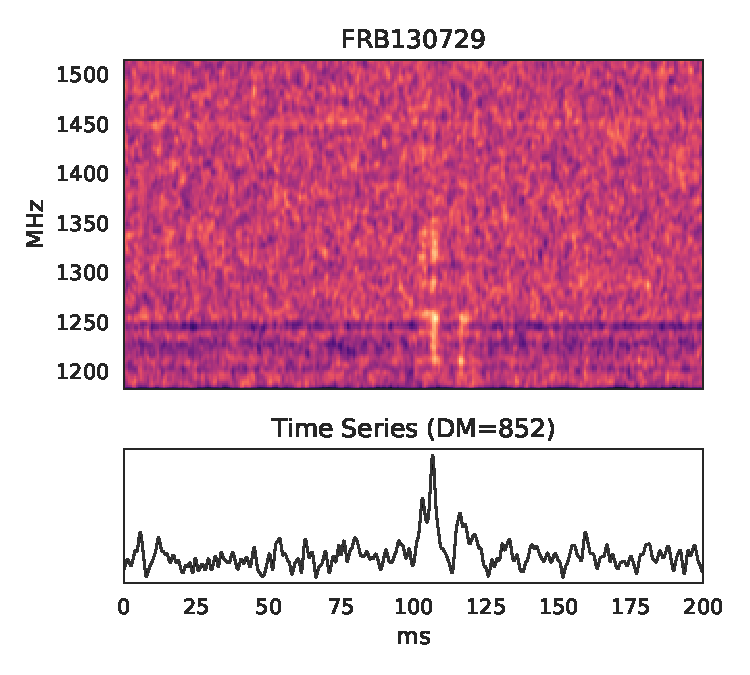
\includegraphics[width=1.0\linewidth]{figures/FRB130729.pdf}
    \caption{FRB130729 dedispersed with a DM of 852~pc~cm$^{-3}$, this is
    different from the SNR-maximized DM of 861~pc~cm$^{-3}$. Using this DM shows
    that the detected FRB has two components distinct components separated by
    approximately 10~ms. Data is presented at the native recorded resolution of
    64~$\mu$s, 390~kHz convolved with a Gaussian smoothing filter of size
    512~$\mu$s, 3.125~MHz.
    }
    \label{fig:FRB130729}
\end{figure}

\subsection{FRB140514}

Detection of FRB140514 was reported in \citep{2015MNRAS.447..246P} and was
reported to have significant circular polarization. But, the flux is primarily
concentrated between 1240~MHz and 1270~MHz. This small fractional bandwidth is
not too different from the ARTEMIS event we have reported earlier.  If this
component is removed, for example if the observation was at a slightly different
frequency, or smaller bandwidth, the detected \gls{snr} drops below 10.
Further, many anthropogenic radio transmitters are circularly polarized. But,
it could also be that there is a plasma lensing effect
\citep{2017ApJ...842...35C} which has been used to explain the variable spectral
index and bandwidth of FRB121102, and FRB140514 is indeed astrophysical.

% FRB140514
% aslxlap07:/local/griffin/data/FRB/FRB140514/FRB140514.ipynb
\begin{figure}
    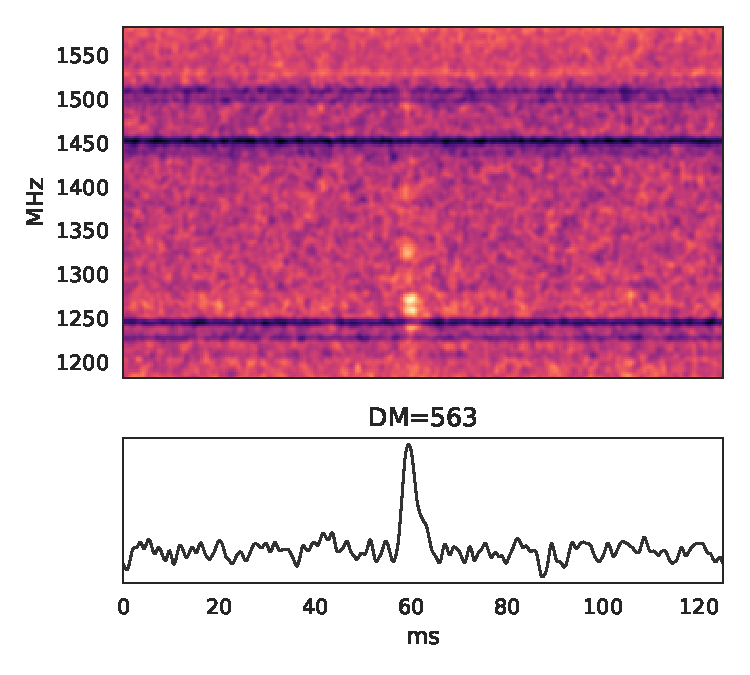
\includegraphics[width=1.0\linewidth]{figures/FRB140514.pdf}
    \caption{The flux of FRB140514 is concentrated in a few, narrow fractional
    bandwidth regions, primarily centred around 1260~MHz.  Data is presented at
    the native recorded resolution of 64~$\mu$s, 390~kHz convolved with a
    Gaussian smoothing filter of size 512~$\mu$s, 3.125~MHz.
    }
    \label{fig:FRB140514}
\end{figure}

\subsection{False-Positive Reporting}

During a search for anomalous signals it should be expected that there are a
number of events reported which are false positives. Such as Perytons
\citep{2011ApJ...727...18B} and the events reported in earlier sections. Events
such as FRB130729 and FRB140514 are on the edge of verifiability. They do not
fit the classic \gls{frb} model but given the available observing and system
information, and lack of an external, anthropogenic explanation they are hard
to discount as not being of astrophysical origin. It is necessary to report
all of these events and to provide as much evidence as possible to explain the
origin of such events.

\section{Verification Tests}

The one-off nature of \glspl{frb} makes it essential that when reporting on a
detection or triggering a follow-up observation that significant due-diligence
is done in order to verify a true-positive detection as much as possible. Over the
past decade of \gls{frb} surveys a number of techniques have been developed to
efficiently filter for dispersed pulses. The vast majority of events are flagged
by \gls{rfi} excisers and setting a sufficiently high minimum \gls{snr}
threshold. This has the effect of creating potential false-negative events (i.e.
FRBs classified as RFI), but is not useful with false-positive detections. The
mystery and rarity of FRBs makes it difficult to differentiate astrophysical FRBs
from local sources based on the dynamic spectrum alone. Thus, additional
information on the observing system should be used to provide robustness to the
detection.

\subsection{Minimum Reporting}

At a minimum, a reasonable detection should be reported with the observed data
made publicly available.  This allows independent verification, and can be used
as input data sets to test pipeline development.  This is different from other
transient detections in that astronomical pointing and observing frequency is
sufficient to do a follow-up observation. If \glspl{frb} are indeed one-off
event, then the detection data is the only data that will ever be available. A
minimum reporting should include:

\begin{enumerate}
    \item Filterbank which fully encompasses the extent of the dispersed pulse.
    \item Time and frequency resolutions, DM, and start time of detection.
    \item Dedispered time series.
    \item Astronomical pointing, observing frequency, and other telescope
    observing parameters.
    \item For a multi-beam system, filterbanks of each beam covering the extent
    of the pulse.
    \item A list (or guide) of software and parameters used to generate
    detections and plots.
\end{enumerate}

These requirements are typically included in past reported \gls{frb} detections.
The last point, a guide on which software was used is often not reported.
Different software and data formats can have slightly different results, such as
the reported \gls{snr} or time definition.  FRBCAT \citep{2016PASA...33...45P}
provides a well-curated repository for this information. The atypical
\glspl{frb} shown in Section \ref{sec:previous_frbs} are from the online data
repositories linked in FRBCAT. Most reported \glspl{frb} detected with Parkes
have publicly accessible data repositories which meet the reporting requirements
stated above. As of this writing, there is no publicly available data for
approximately a quarter of the reported \glspl{frb}. Upon publication of a
detection, this data should be made available.
% FRB110703: dodgy filterbank
% FRB110523, FRB121102, FRB150807, FRB160317, FRB160410, FRB160608, FRB170107,
% FBR170827
% FRB150807: bright, maybe RFI

\subsection{Desirable Reporting}

As has been shown in the previous section there are instrumentational and RFI
sources which can produce the appearance of \glspl{frb}. Minimum reporting is
insufficient for these non-astrophysical detections. These detection were only
excluded with additional understanding of the telescope and observing status.
Primarily this would be to expand the reported data in time before and after the
detected event. Desirable reporting would include:

\begin{enumerate}
    \item Filterbank data which not only encompasses the detected pulse, but
    includes data over a longer time span, e.g. a few minutes before and after
    the detection. If multiple feeds were in use, data from all feeds should be
    made available.
    \item An expected bandpass model, and bandpass model during detection. And,
    the measured gain variation over the observation.
    \item Telescope observing parameters and pointing over the observation,
    including the local (altitude, azimuth) pointing.
    \item A DM-space plot of the detection, along with a negative DM-space
    sampling.
    \item A dispersion fit to the pulse.
    \item Raw voltage or complex spectral data before power detection and
    integration.
\end{enumerate}

Reporting of the bandpass and gain variations, along with a long time data set
allows the state of the telescope to be understood. A deviation from normal
operation, e.g. analogue electronics going into non-linear states, has the
potential to produce spurious events which on a small time-scale can look
FRB-like.

A DM-space plot provides a useful diagnostic to protect against observation
bias. An ideal detection, such as in Figure \ref{fig:dm_time_B1859}, should
appear compact in this space, with no other detections at different trial DMs.

\subsubsection{Multi-site Observations}

Clear evidence for an FRB to be of astrophysical origin is the simultaneous
detection of signal with telescopes at multiple sites. Multiple detectors, such
as in LIGO, are essential for false-positive rejection. Coordinating telescope
observations in logistically difficult, for example many FRB surveys run
commensally during targetted observations, but would prove valuable in reporting
detections.  Further, detection of an FRB at multiple bands would provide
insight into the bandwidth characteristics of the event.

Interferometric arrays provide a similar advantage to multi-site observations.
Detections with individual recievers indicate an event is not due to systematics
such as those in Section \ref{sec:D20161204}. And, the array can be used to
localize the sky position. A detection could still be due to an RFI source local to
the array, though the physical seperation of the elements and interferometric
techniques could be used to determine if the source is in the near field.

\subsubsection{Low-SNR Follow-up Search}

Once a potential detection has been made at a given minimum \gls{snr} threshold,
a second search should be performed focused on a DM range centred on the
SNR-maximzed DM. This search should go to a lower minimum SNR threshold.
Preferably this search would be over the entire observation. This test will
serve to show whether there are additional events, similar to the XAO events,
just below the minimum threshold, or this is a true outlier event.

\subsubsection{Negative DM Sampling}

Current surveys typically search out to extreme \glspl{dm}, in the case of
ALFABURST we search out to a \gls{dm} of 10000~pc~cm$^{-3}$ as the additional
computational cost is minimum. If the \gls{dm}-redshift relation is
approximately correct, searching to such high \glspl{dm} is sufficient to sample
out to the very early universe. We expect an astrophysical source to be
dispersed by a positive \gls{dm} value. As such we do not search for negatively
dispersed pulses. But, \gls{rfi} does show up as both positive and negative
dedispersion detections (Figure \ref{fig:beamo0_80s}). As the dedispersion
search is no longer computationally limited it is possible to search the
negative \gls{dm} space at low additional cost. This would be useful as a
statistical statement about the number of positive versus negative detections to
quantify the amount of \gls{rfi} during a detection. The full negative \gls{dm}
space would not need to be searched, a regular sampling of the space would be
sufficient.

\subsubsection{Dispersion Fitting}

FRB surveys, by design, search for broadband signals which follow a $\nu^{-2}$
cold plasma dispersion relation. A distant astrophysical pulse should follow
this relation, and any deviation from this relation is strong evidence for the
signal being artifically generated, e.g. the XAO repeating event in Section
\ref{sec:xao_event}. This dispersion relation can be tested on the dynamic
spectrum of a potential FRB.

The incoherent dedispersion operation aligns frequency subbands based on such a
frequency-dependent time delay. The dynamic spectrum is averaged in frequency to
produce a time series. Peaks above a threshold S/N are recorded as possible
detections. But, such a detection is not necessarily maximized in S/N with at
the cold plasma dispersion index ($\alpha = -2$). The frequency-dependent delay
of a dispersed pulse can be modelled as
%
\begin{equation}
\Delta t = A \, (\nu_1^{\alpha} - \nu_2^{\alpha}) + \Delta t_0,
\end{equation}
%
where $A$ is the scaling amplitude, for $\alpha = -2$, $A = {\rm DM}$, $\nu_1$
is the reference frequency (usually taken to be the highest frequency subband),
and $\nu_2$ is the observing frequency of a subband.

To perform the fit, the pulse signal needs to be seperated from the noise. This
can be done with various methods. A simple method is to pick the peak flux value
of each subband, that position corresponds to a delay and the flux value is used
as a weight. A more advanced method would be to find the position peak after
correlating the subband with a Gaussian pulse with a width similar to the
detected pulse. In any method, it is useful to exclude subbands where the pulse
is at a low S/N, and limit the maximum delay region to near the predicted
$\nu^{-2}$ delay. The initial parameters for the fit are set to be the original
$\nu^{-2}$ detection parameters.

To produce a reasonable fit and error estimate of the dispersion index
sufficient power needs to be present across a large enough fractional bandwidth.
For example, system such as ALFABURST and ARTEMIS have narrow fractional
bandwidth ($\sim 0.05$) which is insufficient to differentiate between a linear
chirp ($\alpha = -1$) and a cold-plasma dispersed pulse. Similary, this is the
case for a potential FRB that is only detected at significant S/N in a small
fractional bandwidth (e.g. FRB140514).

If the complex voltages are captured during a detection a better dispersion
relation fit can be performed by doing coherent dedispersion. It is often not
practical to store all the unaccumulated voltages during a survey. But, either
detection triggers or short-term storage of the complex voltages be useful for
this test which provides strong evidence for the astrophysical nature of a
pulse.

\subsection{Future Observational Methods}

Beyond detection of more \glspl{frb}, the goals of current surveys are to
localize the source to host galaxies, and detect pulses across broader
bandwidths across the radio spectrum.

Localization requires the use of interferometric arrays. In the case of a
compact array, a high-time resolution correlation matrix is recorded. And, in
the case of \gls{vlbi} the raw complex voltages are recorded, which can be used
to perform coherent dedispersion resulting in a higher resolution (time and
frequency) dynamic spectrum of the pulses.  Related, multi-site coordinated
observations would remove most, if not all, instrumentational and RFI sources of
false-positive detections.

Detection of \glspl{frb} at multiple frequencies not only adds to the scientific
understanding of the sources, but also help to verify that they are
astrophysical.  Due to historical development of receivers for pulsar searches,
most \glspl{frb} have been detected at L-band frequencies. Though, FRB110523
detected with the GBT and the multiple \glspl{frb} detected with UTMOST occurred
at UHF frequencies.  Only FRB121102 has been detected above L-band.  Pulses from
FRB121102 have been detected across a 4 GHz band (4 - 8~GHz) \citep{atel10675}.
Such wide bands show the pulse structure goes beyond the bandwidth of known
source of \gls{rfi} (e.g. modulated RADAR).

\section{Conclusion}

\glspl{frb} are unique astronomical sources from an observational point of view
as so far no follow-up observations have been able to verify a source using a
different telescope or observing frequency, except in the case of FRB121102
which is known to repeat. Thus, it is necessary to provide reasonable evidence
for an astrophysical origin when reporting a detection. 

As the size and number of \gls{frb} surveys continues to increase, one expects
an increase in the number of false-positive detections, even as rejection models
are improved. There is a narrow line between true, astrophysical \glspl{frb} and
false-positive events. Ancillary evidence of the telescope state and observation
provide robust evidence for a true-positive detection. 

Reporting of false-positive events, even if the source is not explained, helps
to improve the robustness of search pipelines against systematics and \gls{rfi}.
Reporting these events also help improve the case for \glspl{frb} being of
astrophysical origin, just as the explanation for Perytons
\citep{2015MNRAS.451.3933P} removed doubt about detections using Parkes.

Though many previously reported \gls{frb} detections have provided sufficient
data and telescope information, more can be provided to present a stronger case
for the astrophysical nature of the detection. Any reported detection at the
minimum should make the observation publicly accessible. Further, as
observing with any radio telescope requires high expert knowledge, it is useful
for the expert observer to include a statement of the telescope status at the
time of a detection.

Current and future surveys which search across large fractional bandwidths, and
localize with interferometric observations will provide further evidence to
associate an \gls{frb} detection with an astrophysical source.

Jupyter notebooks and the filterbanks files are hosted on our
public git
repository\footnote{https://github.com/griffinfoster/terrestrial-frb-letter}.

\bibliographystyle{mnras}
\bibliography{frb-detections} 

% Don't change these lines
\bsp	% typesetting comment
\label{lastpage}
\end{document}

% End of mnras_template.tex
